% 1. Архитектура вычислительных систем. Основные понятия

\chapter{Архитектура вычислительных систем. Основные понятия}

\section{Определение архитектуры ВС}

Понятие архитектуры трактуется весьма разнообразно в различных областях человеческой деятельности. Отсутствует однообразие трактовки и архитектуры вычислительной системы

\textbf{Определение 1.} \textit{Архитектура ВС} --- концептуальная структура вычислительной машины, определяющая проведение обработки информации и включающая методы преобразования информации в данные и принципы взаимодействия технических средств и программного обеспечения.

\textbf{Определение 2.} \textit{Архитектура ВС} --- абстрактное представление ЭВМ, отражающее её структурную, схемотехническую и логическую организацию.

\textbf{Определение 3.} \textit{Архитектура ВС} --- множество взаимосвязанных компонент ЭВМ, включающих: программное обеспечение (software), аппаратное обеспечение (hardware), алгоритмическое обеспечение (brainware), специальное микропрограммное обеспечение (firmware) + система (структура), поддерживающая слаженное функционирование перечисленного.

\textbf{Определение 4.} \textit{Архитектура ВС} --- абстрактное многоуровневое представление физической системы с точки зрения программиста с закреплением функций за каждым уровнем и установлением интерфейса между уровнями.

\textbf{Структура} (от лат. structūra - “строение”) - внутреннее устройство чего-либо. Внутреннее устройство связано с категориями целого и его частей.

Многообразие этого понятия отражается в возможных вариантах критериев классификации архитектрур ВС, среди которых можно выделить:

\begin{itemize}
    \item уровень восприятия;
    \item предметная ориентацию (специализацию);
    \item структурную поддержку
    \item парадигму программирования
\end{itemize}

\subsection{Уровень восприятия}

Многоуровневость обуславливатеся тем, что компьютеры предназначены для программирования, а архитектурные уровни выделяются для повышения эффективности процесса разработки ПО, для преодоления семантического разрыва между предметной областью и реальным исполнителем, предоставляющим архитектуру на уровне системы команд. То есть система воспринимается через ее входной язык программирования, обеспечивающий или написание кода или демонстрирующий функционирование на уровне отдельных внутренних подсистем, поддерживающих выполнение вычислительных процессов. Эта многоуровневость по Э.~Танненбауму~\cite{Tannenbaum-2017} представлена на рисунке~\ref{definition-01}.

\begin{figure}[htbp]
  \centering
  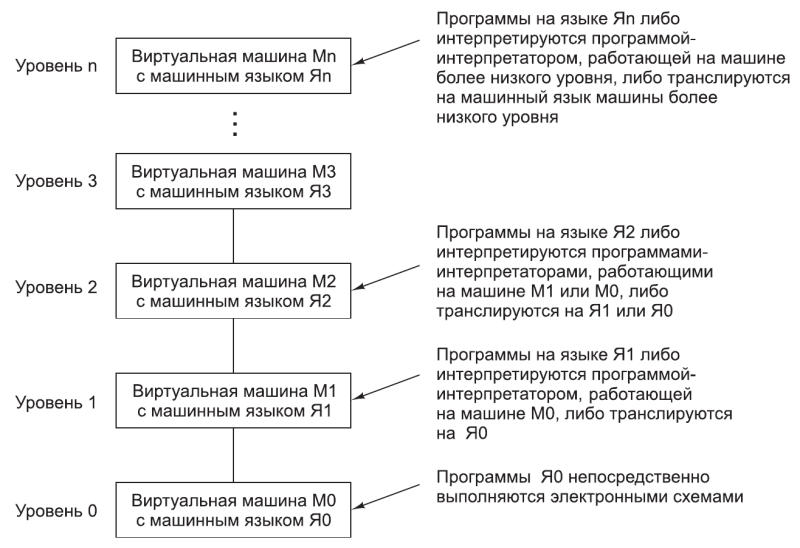
\includegraphics[width=1.0\textwidth]{img/definition-01.png}
  \caption{Понятие многоуровневости архитектуры по Э.\,Танненбауму}
  \label{definition-01}
\end{figure}

Он также приводит конкретную иеррархию уровней, построенную по этой схеме, которая приведена на рисунке~\ref{base-02}.

\begin{figure}[htbp]
  \centering
  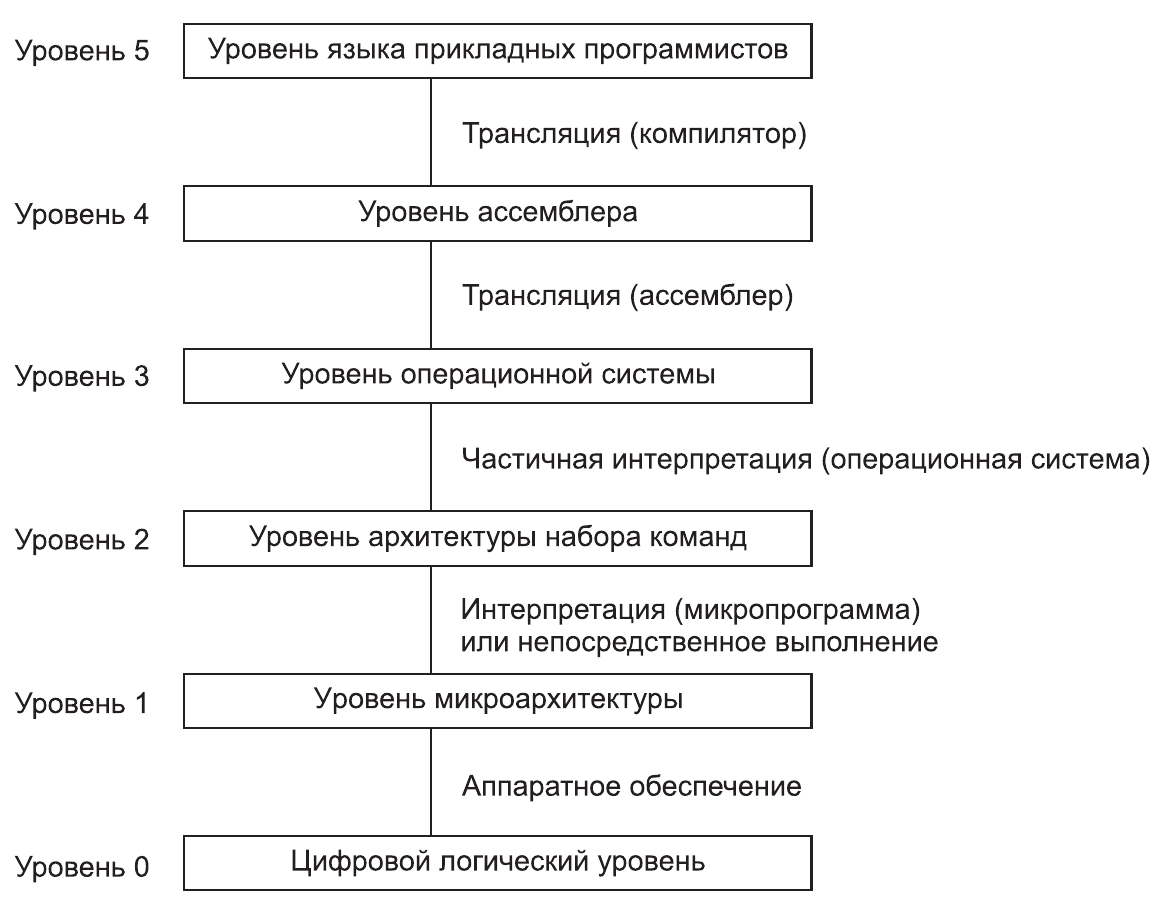
\includegraphics[width=1.0\textwidth]{img/base-02.png}
  \caption{Многоуровневая архитектура ВС по Э.\,Танненбауму}
  \label{base-02}
\end{figure}

Вместе с тем следует отметить, что можно предствить и большую детализацию уровней, что обуславливается спецификой использования каждого из них в современном процессе разработки программного обеспечения и широкого использования промежуточных виртуальных архитектур. Она будет выглядеть следующим образом:

\begin{itemize}
    \item Уровень предметно--ориентированных (специализированных) языков (Norma, ANTLR, GPSS, Prolog, Cmake...)
    \item Уровень универсальных языков прикладного программирования (Java, Kotlin, C\#, Python, Go, JS...)
    \item Уровень языков ориентированных на системное программирования (C, C++, Rust...)
    \item Уровень промежуточных языков (LLVM, MSIL, JavaVM...)
    \item Уровень ассемблера
    \item Уровень операционной системы
    \item Уровень архитектуры набора команд
    \item Уровень микроархитектуры
    \item Цифровой логическиий уровень
\end{itemize}

Весьма часто в профессиональной деятельности возникает необходимость ориентации в как в прикладных аспектах решаемой задачи так и в эффективном отображениии на используемую ВС. То есть в рассмотрении решаемой задачи с позиций нескольких архитектурных уровней восприятия. Это может быть связано со следующими факторами:

\begin{itemize}
    \item Многие классы задач требуют понимания и использования разнообразных по уровню компьютерных архитектур.
    \item Часто в компаниях перебрасывают программистов с одного проекта на другой. При этом изменяются характеристики языковых и инструментальных средств, определяющих специфику уровней архитектуры.
    \item Некоторые направления предметной области изменяются за счет автоматизации, отсутствия спроса и по другим причинам. Это ведет к необходимости переориентации на другие задачи, зачастую меняющие уровень используемой компьютерной архитектуры.
    \item Незнание методов и подходов других архитектурных уровней зачастую ведет к неэффективному решению поставленной задачи за счет неправильно выбора инструментов, которые соответствуют текущим знаниям разработчика, но не соответствуют архитектурному уровню решаемой задачи. При этом возможны:
    \begin{itemize}
        \item несоответствие вниз, когда незнание более низких уровней ведет к потере эффективности при работе программы на реальной ВС;
        \item несоответствие вверх, когда процесс разработки программного обеспечения становится менее эффективным, за счет неправильного выбора инструментов.
    \end{itemize}
\end{itemize}

Каждый архитектурный уровень не обязательно должен поддерживаться соответствующими инструментальными средствами. Зачастую один и тот же инструмент, ориентированный на конкретный архитектурный уровень, обеспечивает поддержку как вышележащих, так и нижележащих уровней. Подобными качествам обладает практически любой язык программирования. В качестве примера можно привести C++. Несмотря на то, что он в основном позиционируется как язык системного программирования, наличие таких абстракций как функции и классы позволяют создавать библиотеки, которые могут позиционироваться как поддержка вышестоящих уровней. В качестве примера покрытия различных уровней можно привести:

\begin{itemize}
    \item поддержка предметно--ориентированного или специализированного программирования с использованием библиотек SFML, SDL и других;
    \item поддержка универсального программирования на прикладном уровни, реализуемого с использованием стандартной библиотеки языка или библиотеки Boost;
    \item на уровне системного программирования непосредственно используются средства самого языка и ряда специализированных библиотек;
    \item поддержка уровня системы команд обеспечивается встроенным ассемблером.
\end{itemize}
